\section{PROPOSED FRAMEWORK (MAUI) BASED ON BOOLEAN SATISFIABILITY (SAT)}
\label{sec:framework}
%(1) TVA, DCC are equal
\begin{comment}
There exist two basic idea in the proposed framework for aging tolerance. The two idea are based on time-borrowing, so as to mitigate the aging-induced performance degradation of logic network. The first idea is based on aging manipulation by inserting \textit{duty-cycle converters} (DCCs) in the existing clock tree. The second idea is based on V\textsubscript{th} assignment of clock buffers by inserting the technology leaders in the clock tree. This way, we can intentionally create aging-induced and tech-induced clock skews, which can compensate for the performance degradation of the logic circuit based on time borrowing. We formulate the problem using Boolean satisfiability (SAT) and thanks to the efficiency of existing SAT solvers, the optimal solution can be obtained efficiently. The end result of this formulation is the locations (in the existing clock tree) of DCCs and technology leaders such that, when aging-induced and tech-induced clock skews are considered, the required clock period of the given circuit under $n$-year BTI is minimized. The clock period can be minimized since the performance degradation of the logic circuit is \enquote{tolerated} as a result of useful (aging-induced and tech-induced) clock skews. The minimum required clock period thus implies maximum level of aging tolerance. Note that, as mentioned in \ref{sec:motivate:exp2}, we re-assign V\textsubscript{th} of clock buffers, based on the insertion of technology leader\footnote{Technology leader is an imaginary location instead of a physical gate such as DCC. It indicates the location where we begin assigning new-V\textsubscript{th} to clock buffers toward flip-flops, but exclude flip-flops (i.e., the V\textsubscript{th} of flip-flops will not be re-assigned to new counterpart.}, from which we begin assigning new-V\textsubscript{th} to the downstream\footnote{The downstream clock buffers are those between imaginary technology leader and flip-flops. We use the adjective "downstream" to describe the clock buffers, based on the direction that clock signal pass toward (i.e., clock signal is generated from clock source, passes through clock buffers, and finally arrives at flip-flops).} clock buffers toward flip-flops.
\end{comment}

%(1) DATE 2018
The basic idea of our MAUI framework for aging tolerance is to insert \textit{duty-cycle converters} (DCCs) in the existing clock tree, so as to intentionally create aging-induced clock skews which can compensate for the performance degradation of the logic circuit based on time borrowing. We formulate the problem using Boolean satisfiability (SAT) and thanks to the efficiency of existing SAT solvers, the optimal solution can be obtained efficiently. The end result of this formulation is the locations (in the existing clock tree) to insert DCCs such that, when aging-induced clock skews are considered, the required clock period of the given circuit under $n$-year BTI is minimized. Note that the clock period can be minimized since the performance degradation of the logic circuit is \enquote{tolerated} as a result of useful aging-induced clock skews. The minimum required clock period thus implies maximum level of aging tolerance.

%\begin{figure*}
%	\centering
%	\begin{minipage}[b]{.45\textwidth}
%		\centering
%		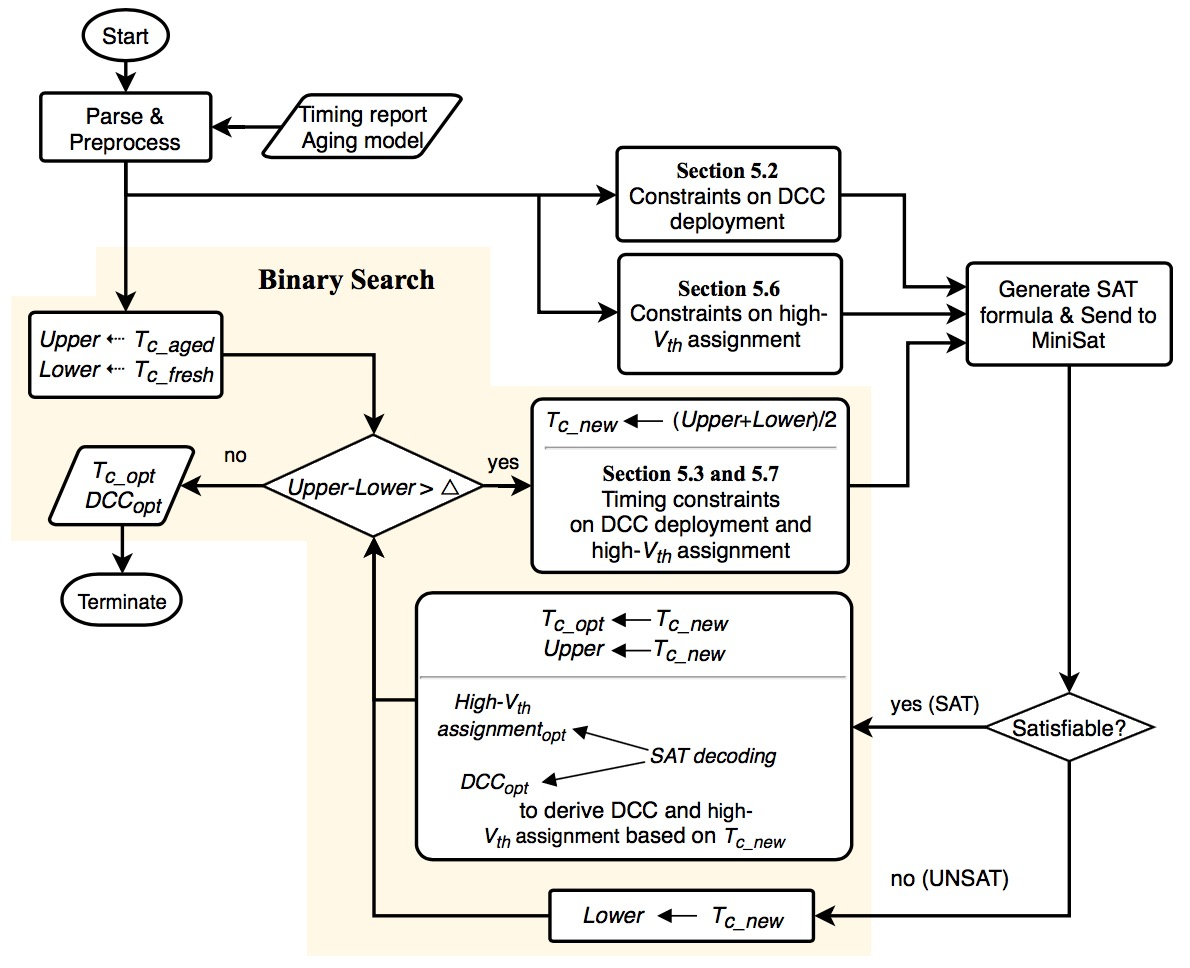
\includegraphics[width=0.9\columnwidth]{Flow_chart.png}
%		\caption{The overall flow of MAUI}
%		\label{fig:flow}
%	\end{minipage}
%	\hspace{1cm}
%	\begin{minipage}[b]{.45\textwidth}
%		\centering
%		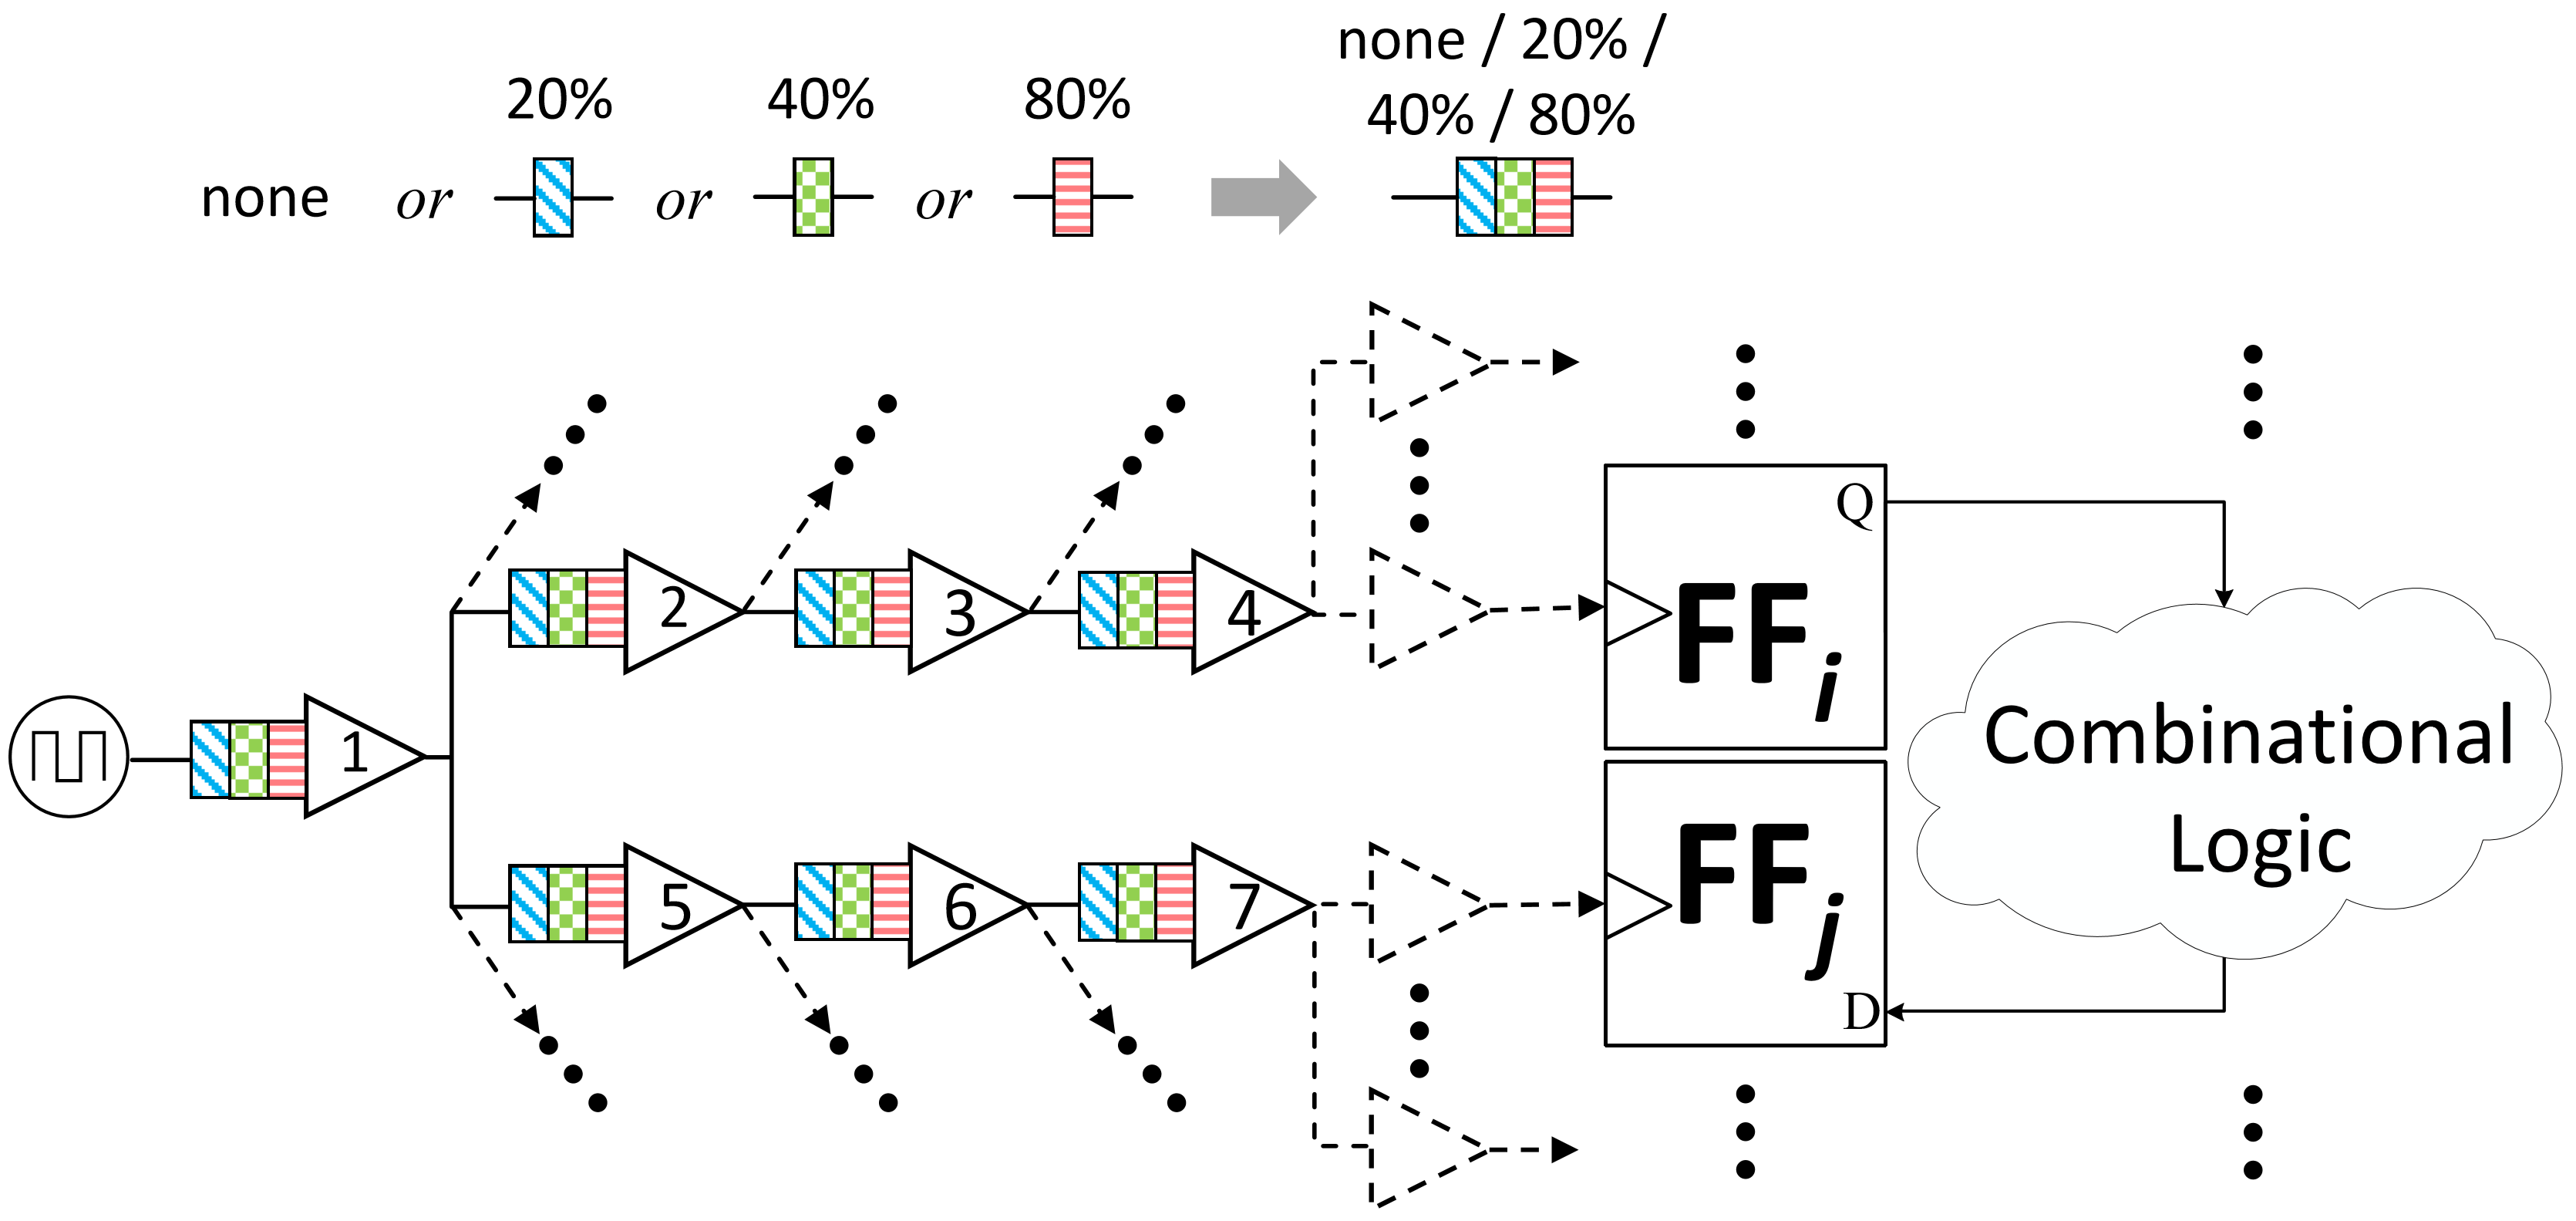
\includegraphics[width=0.9\columnwidth]{All_types_of_DCCs.png}
%		\caption{Generalized DCC insertion for a target pair of flip-flops}
%		\label{fig:dcctype}
%	\end{minipage}
%\end{figure*}

\begin{figure}
	\centering
	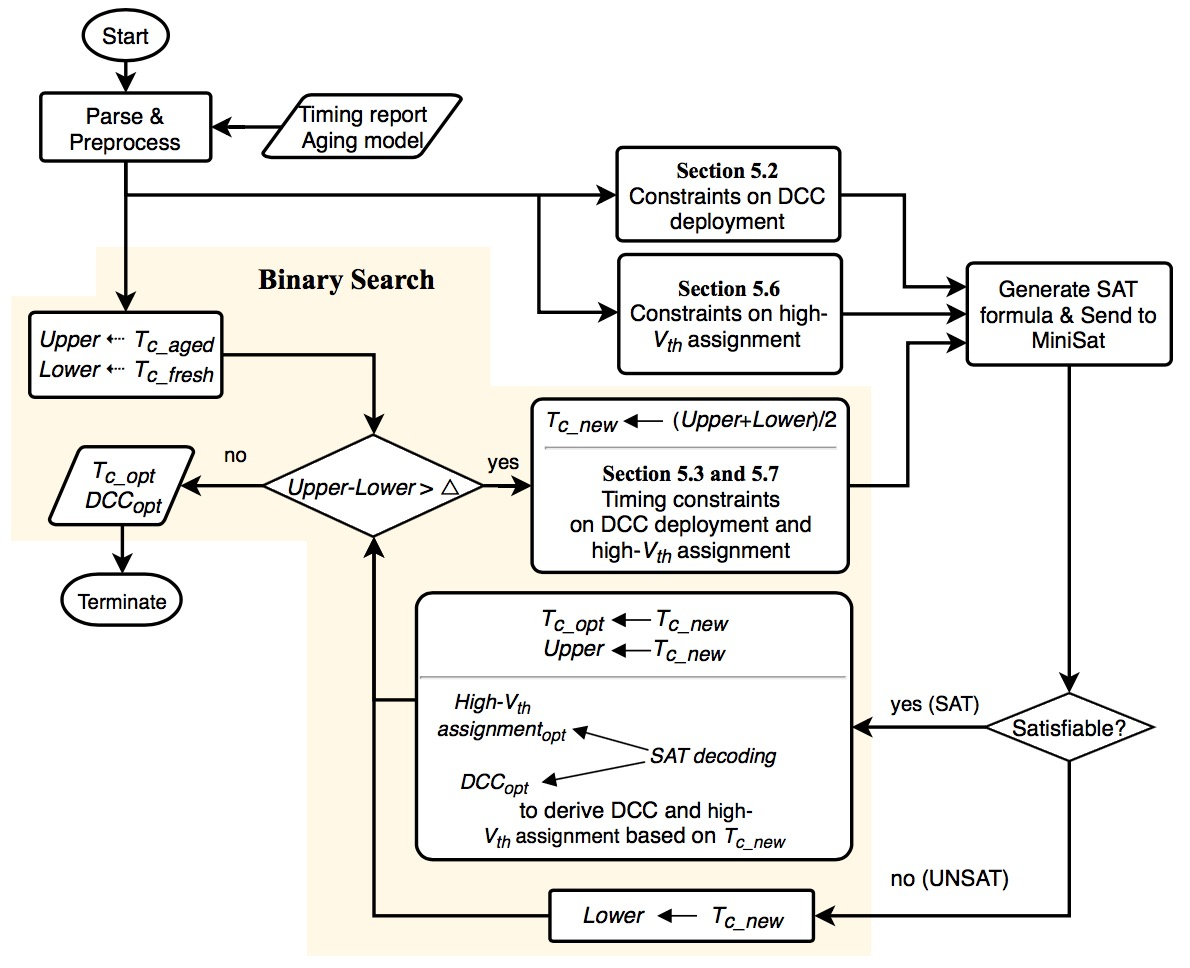
\includegraphics[width=0.9\columnwidth]{Flow_chart.png}
	\caption{The overall flow of MAUI}
	\label{fig:flow}
\end{figure}

%(2) TVA, DCC are equal
\begin{comment}
The overall flow of our framework is depicted in Figure~\ref{fig:flow}, where a binary search for the minimum clock period ($T_c$) is involved. Formulated based on SAT, the key of our framework is to represent the problem in \textit{conjunctive normal form} (CNF). A CNF representation is a conjunction of one or more clauses, where each clause is a disjunction of one or more Boolean variables. In the sequel, Section~\ref{subsec:eddcd} explains how the proposed problem of DCC and technology leader deployment/insertion is encoded by Boolean variables. Section~\ref{subsec:dccccc} and Section~\ref{subsec:tccc} describe three major components, DCC constraints, HTV leader constraint and timing constraints, for our SAT-based formulation and how they are translated into legal SAT formula, i.e., CNF representation.
\end{comment}

%(2) DATE 2018
The overall flow of our MAUI framework is depicted in Figure~\ref{fig:flow}, where a binary search for the minimum clock period ($T_c$) is involved. Formulated based on SAT, the key of our framework is to represent the problem in \textit{conjunctive normal form} (CNF). A CNF representation is a conjunction of one or more clauses, where each clause is a disjunction of one or more Boolean variables. In the sequel, Section~\ref{subsec:eddcd} explains how the proposed problem of DCC deployment/insertion is encoded by Boolean variables. Section~\ref{subsec:dccccc} and Section~\ref{subsec:tccc} describe two major components, DCC constraints and timing constraints, for our SAT-based formulation and how they are translated into legal SAT formula, i.e., CNF representation.

\afterpage{
\begin{figure}
	\centering
	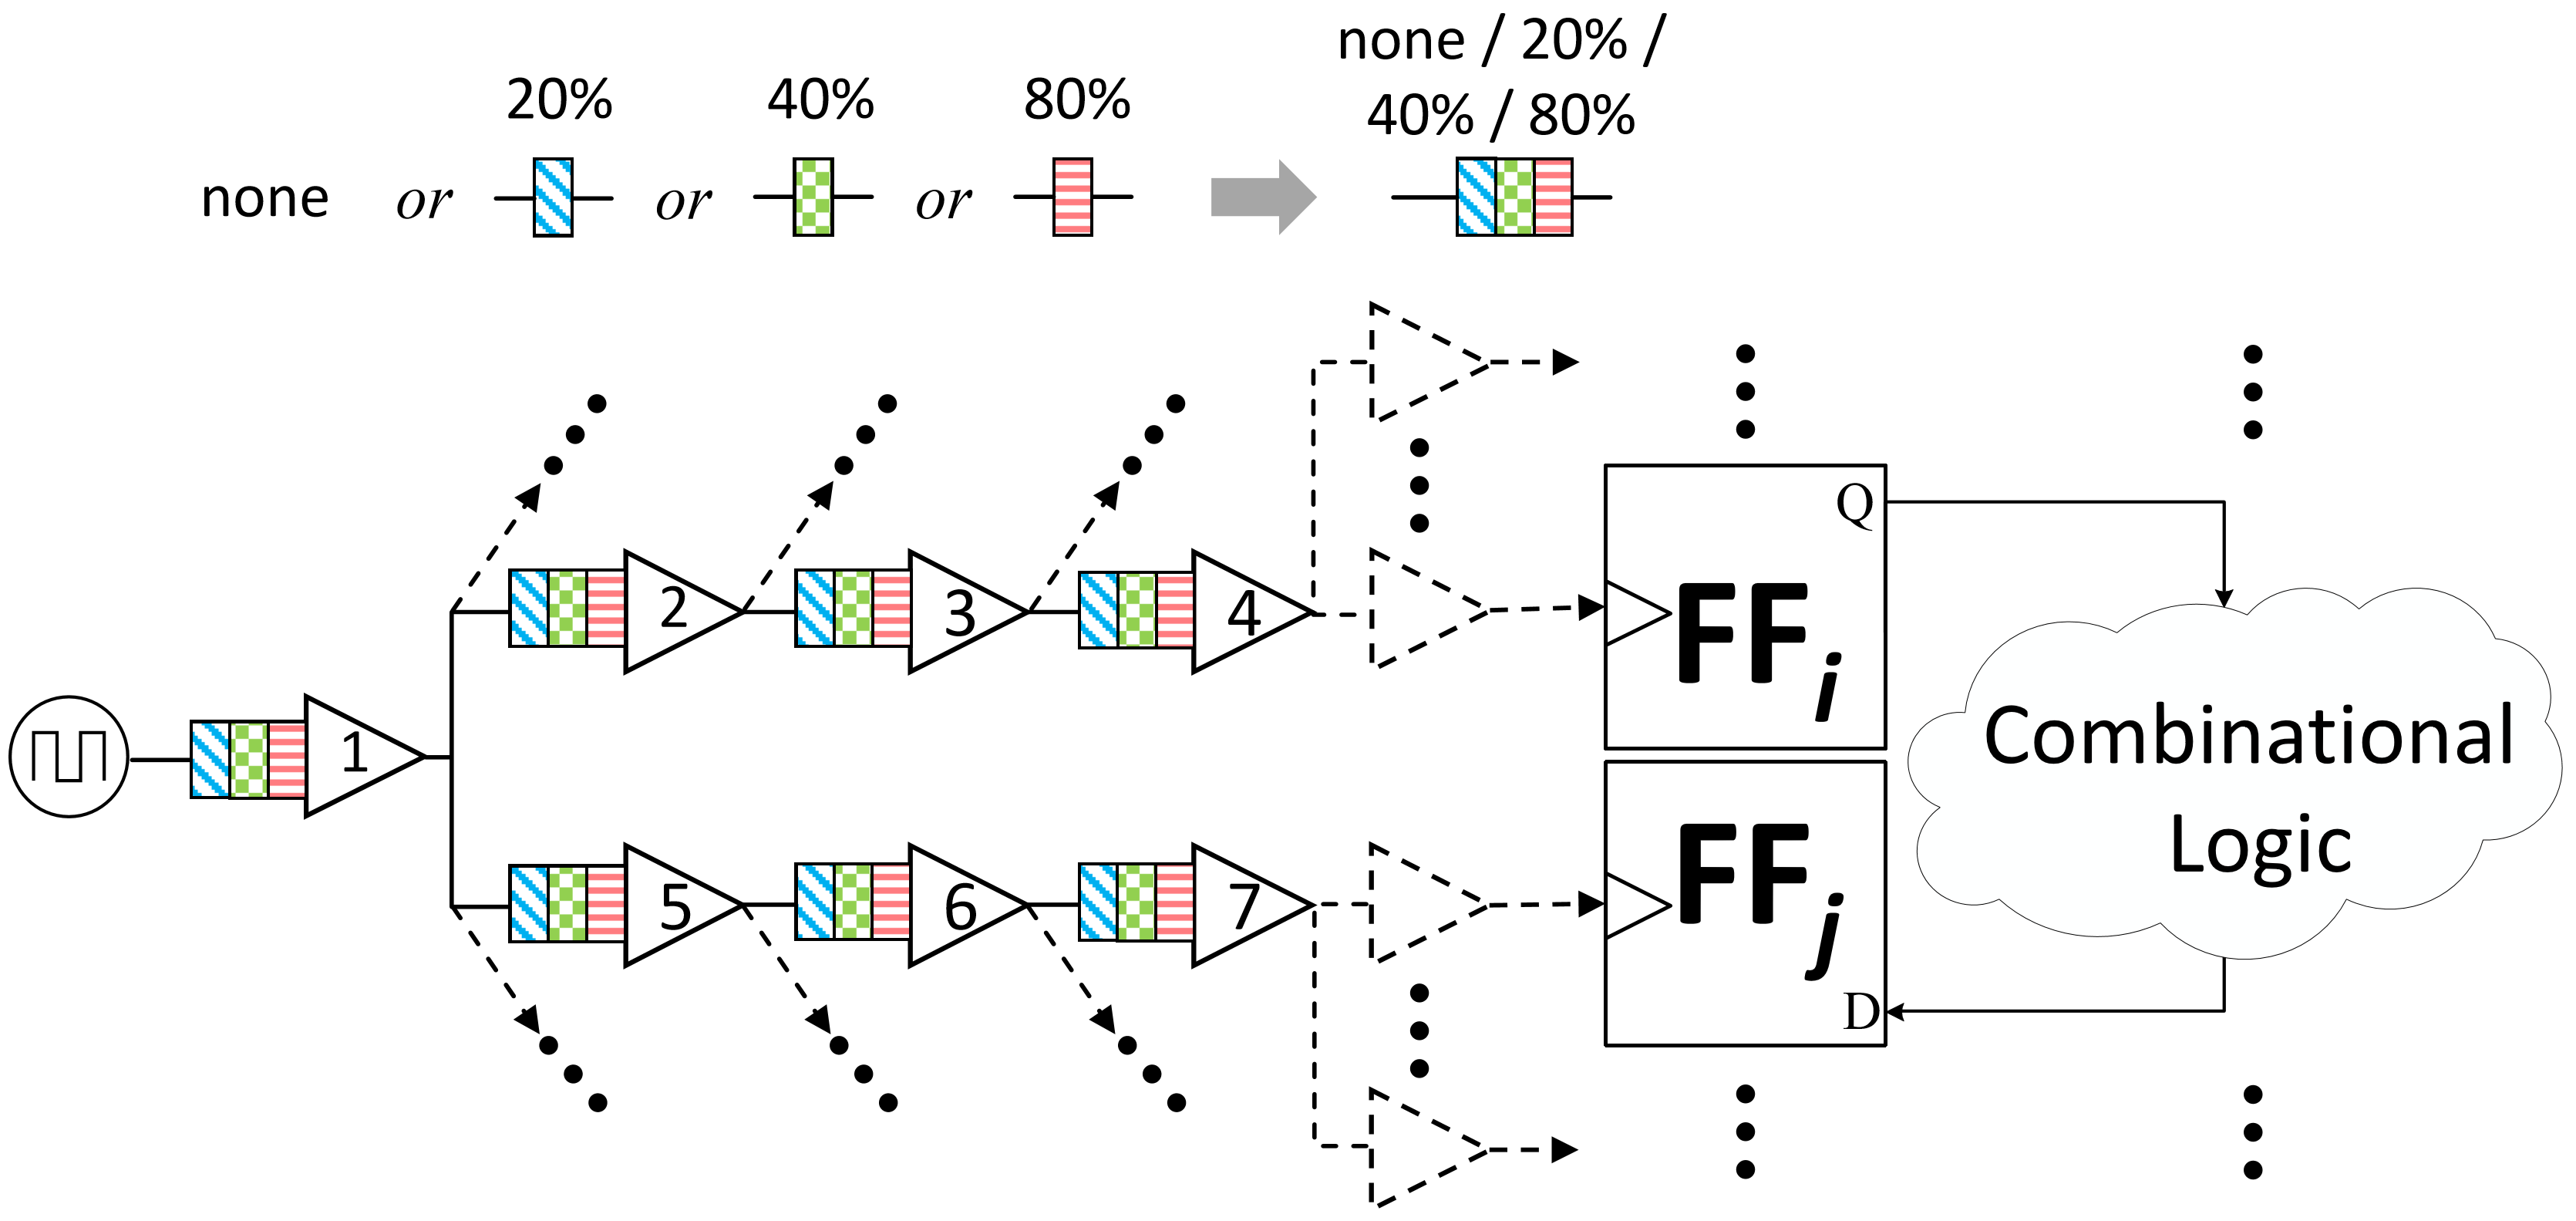
\includegraphics[width=0.9\columnwidth]{All_types_of_DCCs.png}
	\caption{Generalized DCC insertion for a target pair of flip-flops}
	\label{fig:dcctype}
\end{figure}
}

%(3) TVA, DCC are equal
\begin{comment}
\subsection{Encoding for DCC and Technology Leader Deployment}
\label{subsec:eddcd}
The deployment/insertion problem of DCC and technology leader needs to be encoded into Boolean representation before being transformed into a SAT-based formulation. Assume that a total of $N$ types of DCCs can be chosen. Including the DCC-free case where no DCC is inserted, there are ($N$ + 1) possibilities of DCC insertion for each clock buffer. Furthermore, we also assume that a total of $M$ types of technology leaders can be chosen. Including the nominal case where no technology leader is inserted, there are ($M$ + 1) possibilities of technology leader insertion for each clock buffer. Note that, when a DCC/technology leader is inserted, it is inserted at the input of a buffer. We denote a clock buffer by $p\left(1 \leq p \leq P\right)$ where $P$ is the number of buffers. For each buffer, Boolean variables $B_{p,q}\left(1 \leq p \leq P, 1 \leq q \leq Q = \lceil \lg (N + 1)(M + 1)\rceil \right)$ are introduced where $\left\{B_{p,1}, B_{p,2},\dotsc, B_{p,Q}\right\}$ encode the aforementioned ($N$ + 1)($N$ + 1) possibilities of DCC insertion at the input of buffer $p$.
\end{comment}

%(3) DATE 2018
\subsection{Encoding for DCC Deployment}
\label{subsec:eddcd}
The problem of DCC deployment/insertion needs to be encoded into Boolean representation before being transformed into a SAT-based formulation. Assume that a total of $N$ types of DCCs can be chosen. Including the DCC-free case where no DCC is inserted, there are ($N$ + 1) possibilities of DCC insertion for each clock buffer. Note that, when a DCC/HTV leader is inserted, it is inserted at the input of a buffer. We denote a clock buffer by $p\left(1 \leq p \leq P\right)$ where $P$ is the number of buffers. For each buffer, Boolean variables $B_{p,q}\left(1 \leq p \leq P, 1 \leq q \leq Q = \lceil \lg (N + 1)\rceil \right)$ are introduced where $\left\{B_{p,1}, B_{p,2},\dotsc, B_{p,Q}\right\}$ encode the aforementioned ($N$ + 1) possibilities of DCC insertion at the input of buffer $p$.

%(4) DATE 2018
Without loss of generality, we assume $N$ = 3 (types of DCCs) and they are 20\%, 40\%, and 80\% DCCs, as shown in Figure~\ref{fig:dcctype}. Therefore, two Boolean variables are used for encoding four possibilities of DCC insertion at the input of any buffer. The four possibilities can be encoded as follows:

%(5) DATE 2018
\begin{tabular}{ l c }
  DCC type: & $\left\{B_{p,2},B_{p,1}\right\}$ \\
  (1)\quad None: & \{0,0\} \\
  (2)\quad 20\%: &  \{0,1\} \\
  (3)\quad 40\%: &  \{1,0\} \\
  (4)\quad 80\%: &  \{1,1\} \\
\end{tabular}

\afterpage{
\begin{figure*}
    \centering
    \subfigure[Case 2-1: one DCC on the common clock path (e.g., at buffer 1)]{
    	\label{fig:sub:dcci1}
        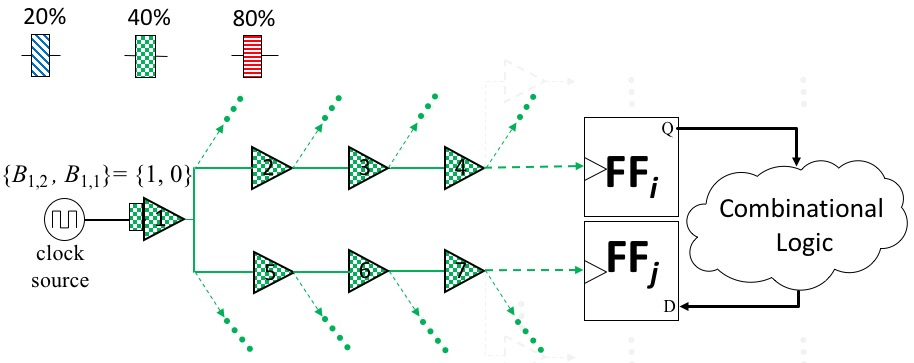
\includegraphics[width=0.9\columnwidth]{A_examlpe_of_DCC_placement1.png}
    }
    \hspace{1cm}
    \subfigure[Case 2-2: one DCC on one of the divergent clock paths, or class 3: two DCCs, one on each of the divergent clock paths]{
    	\label{fig:sub:dcci2}
        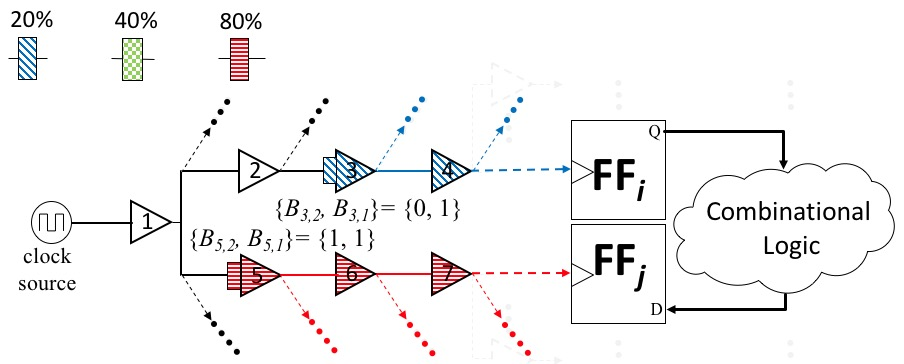
\includegraphics[width=0.9\columnwidth]{A_examlpe_of_DCC_placement2.png}
    }
    \caption{Examples of DCC insertion}
    \label{fig:dccinsert}
\end{figure*}
}

For example, in Figure~\ref{fig:sub:dcci2}, a 20\% DCC and an 80\% DCC are inserted at buffer 3 and buffer 6, respectively. Therefore, $\left\{B_{3,2}, B_{3,1}\right\}$ = \{0, 1\}, $\left\{B_{5,2}, B_{5,1}\right\}$ = \{1, 1\}, and $\left\{B_{p,2}, B_{p,1}\right\}$ = \{0, 0\} for $p$ = 1, 2, 4, 6 or 7.

The 20\% DCC will mitigate the aging of buffer 3 and its downstream buffers, while the 80\% DCC will aggravate the aging of buffer 6 and its downstream buffers. It can be found that, if a DCC is deployed deep in the clock tree (i.e., close to the flip-flops), the number of buffers affected is limited and thus the overall impact of aging mitigation/aggravation on $C_i$/$C_j$ may be insignificant, which diminishes the benefit from deploying DCCs for aging tolerance. To avoid this phenomenon, we set a rule of prohibiting DCC deployment at a clock tree level larger/deeper than a specified boundary. This rule also greatly reduces the complexity of our SAT-based formulation because a significant fraction of buffers are excluded from being considered for DCC deployment. For example, in Figure~\ref{fig:dcctype}, those dashed buffers and their downstream buffers are excluded. 

%(2) B
\subsection{DCC Constraints and Corresponding Clauses}
\label{subsec:dccccc}

Figure~\ref{fig:dcctype} shows a generalized example of DCC insertion for a pair of flip-flops (\ce{FF_i} and \ce{FF_j}) where there exist aging-critical paths from \ce{FF_i} to \ce{FF_j}. A path is defined as an aging-critical path if, in the presence of aging, it is possible to determine the clock period of the circuit. Every pair of flip-flops between which there exist aging-critical paths needs to be considered and here, we use this generalized example to illustrate our SAT-based formulation.

In Figure~\ref{fig:dcctype}, buffers 1 $\hyphen$ 7 are candidate locations for DCC insertion and according to the encoding scheme explained in Section~\ref{subsec:eddcd}, two Boolean variables are introduced for each of the seven buffers to encode four possibilities of DCC insertion. Considering all seven buffers, there are a total of 16,384 (= $4^7$) possibilities, just for this pair of flip-flops. This makes the formulation based on SAT intractable due to clause explosion. Therefore, we set up the following constraint on DCC insertion: \\ \\
\textbf{\uline{DCC constraint: At most one DCC on a single clock path (from the clock source to one of the flip-flops)}}

In order to ensure no more than one DCC on any clock path, we can use the Boolean variables introduced for DCC insertion, i.e., $B_{p,q} \left(1 \leq p \leq P, 1 \leq q \leq Q = \lceil \lg (N + 1) \rceil \right)$, to generate some clauses which suppress the occurrence of having two DCCs on a clock path. Consider buffer 2 (encoded by $\left\{B_{2,2}, B_{2,1}\right\}$) and buffer 3 (encoded by $\left\{B_{3,2}, B_{3,1}\right\}$) in Figure~\ref{fig:dcctype}. If there is a DCC at buffer 2 (i.e., $\{B_{2,2}, B_{2,1}\} \not\equiv \{0, 0\}$), then there must no DCC at buffer 3 (i.e., $\{B_{3,2}, B_{3,1}\} \equiv \{0, 0\}$), and vice versa. The constraint can be formally written as:
\begin{gather*}
\left(\{B_{2,2}, B_{2,1}\} \equiv \{0, 0\}\right) \lor \left(\{B_{3,2}, B_{3,1}\} \equiv \{0, 0\}\right)
\end{gather*}
Next, it can be translated into 4 CNF clauses:
\begin{gather*}
\mbox{\fontsize{7}{8.4}\selectfont ($\neg B_{2,1}\lor\neg B_{3,1}$) $\land$ ($\neg B_{2,1}\lor\neg B_{3,2}$) $\land$ ($\neg B_{2,2}\lor\neg B_{3,1}$) $\land$ ($\neg B_{2,2}\lor\neg B_{3,2}$)} 
\end{gather*}

Any pair of buffers along a single clock path should be constrained in this way. Among buffers 1 $\hyphen$ 7 in Figure~\ref{fig:dcctype}, there are 12 pairs: $\langle1, 2\rangle$, $\langle1, 3\rangle$, $\langle1, 4\rangle$, $\langle1, 5\rangle$, $\langle1, 6\rangle$, $\langle1, 7\rangle$, $\langle2, 3\rangle$, $\langle2, 4\rangle$, $\langle3, 4\rangle$, $\langle5, 6\rangle$, $\langle5, 7\rangle$, $\langle6, 7\rangle$. Each pair translates to 4 clauses and a total of 48 clauses will be generated accordingly.

With DCC constraints and corresponding clauses, we can drastically reduce the possibilities of DCC insertion to be formulated. In the above example where 48 clauses associated with DCC constraints are generated, the number of possibilities drops from 16,384 to 103. In the next subsection, we describe what the 103 possibilities are and how they are translated into the final CNF representation.

%(3) C
\subsection{Timing Constraints and Corresponding Clauses}
\label{subsec:tccc}
Given a pair of flip-flops, if there exists one logic path between them, the timing (i.e. setup-time and hold-time) constraints must be met based on the inequalities~(\ref{eq:tsu}) and~(\ref{eq:th}). Different types of DCCs reveal different aging influence on clock latency. Consider the lifespan specification of 10 years in Figure~\ref{fig:sub:dcci2}: the delay of each clock buffer is changed after 10 years. The clock latency of \ce{FF_i} (i.e., $C_i$) is the sum of clock buffer delays from clock source to \ce{FF_i}: \\
$C_i = \tau_1 + \tau_2 + \tau_3 + \tau_4 +\dotsb$ and \\
$C_j = \tau_1 + \tau_5 + \tau_6 + \tau_7 +\dotsb$, \mbox{\fontsize{9}{10.8}\selectfont where $\tau_k$ is the delay of buffer $k$.}\\
Consider aging effects on $C_i$ and $C_j$: \\
$C_{i\_aged} = 1.13 \times \left(\tau_1 + \tau_2\right) + 1.09 \times \left(\tau_3 + \tau_4 + \dotsb\right)$ and \\
$C_{j\_aged} = 1.13 \times \tau_1+ 1.16 \times \left( \tau_5 + \tau_6 + \tau_7 + \dotsb \right)$, where $C_{i\_aged}$ and $C_{j\_aged}$ denote aged $C_i$ and $C_j$, respectively.

Next, we apply Equations~(\ref{eq:tsu}) and~(\ref{eq:th}) to check whether timing constraints will be violated under this DCC deployment.\\ \\
\textbf{\uline{Timing constraint: No existence of timing violation}}

Given one clock period $T_c$ derived by binary search, one aging-critical path, and its associated clock network, all possible DCC deployments can be classified into 3 classes according to the number of DCCs used. Furthermore, due to the aforementioned DCC constraints, the SAT solver will only output a DCC deployment where there does not exist more than one DCC along any clock path. Thus, in the following discussion, the deployment with more than one DCC along a single clock path can be ignored. In each class, if the DCC deployment causes a timing violation within 10 years (i.e., the lifespan specification), then the deployment will be transformed into CNF clauses, such that the solver will not output the deployment as results. Here, we explain the generation of CNF clauses by using the example in Figure~\ref{fig:dccinsert}.

\begin{class}
\label{class:c1}
No DCC is inserted on either clock path

Consider the situation that no DCC is inserted at buffers 1 $\hyphen$ 7. If it causes a timing violation along the aging-critical path within 10 years, then the Boolean representation of the deployment,
\begin{gather*}
\left(\{B_{1,2}, B_{1,1}\} \equiv \{0, 0\} \right) \land \left( \{B_{2,2}, B_{2,1}\} \equiv \{0, 0\} \right) \land \dotsb \\
\land \left( \{B_{7,2}, B_{7,1}\} \equiv \{0, 0\} \right),
\end{gather*}
equivalent to the following CNF clause:
\begin{gather*}
\left(B_{1,2} \lor B_{1,1} \lor B_{2,2} \lor B_{2,1} \lor \dotsb \lor B_{7,2} \lor B_{7,1} \right),
\end{gather*}
should be generated such that the solver will not output the corresponding deployment in the result if the CNF is satisfiable. In this case, a total of 1 CNF clause is generated.
\end{class}
\begin{class}
\label{class:c2}
Inserting one DCC

This class can be further classified into 2 sub-classes based on the location of inserted DCCs. \\
\textit{Class 2-1:} Inserting one DCC on the common clock path

In Figure~\ref{fig:dccinsert}, buffer 1 is on the common clock path. Consider the DCC insertion shown in Figure~\ref{fig:sub:dcci1}: if the insertion of a 40\% DCC at buffer 1 causes a timing violation within 10 years, then the Boolean representation of the DCC deployment, $\left(\{B_{1,2}, B_{1,1}\} \equiv \{1, 0\} \right) \land \left( \{B_{2,2}, B_{2,1}\} \equiv \{0, 0\} \right) \land \dotsb \land \left( \{B_{7,2}, B_{7,1}\} \equiv \{0, 0\} \right)$, equivalent to the following clause: $\left(\neg B_{1,2} \lor B_{1,1} \lor B_{2,2} \lor B_{2,1} \lor \dotsb \lor B_{7,2} \lor B_{7,1} \right)$, should be generated such that the solver will not output the deployment in the result if the CNF is satisfiable. Given that there are 3 choices of DCCs, a total of 3 CNF clauses will be generated in the worst case. \\
\textit{Class 2-2:} \mbox{\fontsize{9}{10.8}\selectfont Inserting one DCC on one of the divergent clock paths}

This class targets buffers 2, 3, 4, 5, 6, 7. If the insertion of a 20\% DCC at buffer 3 causes a timing violation within 10 years, then the Boolean representation of the DCC deployment, $\left(\{B_{3,2}, B_{3,1}\} \equiv \{0, 1\} \right) \land \left( \{B_{1,2}, B_{1,1}\} \equiv \{0, 0\} \right) \land \dotsb \land \left( \{B_{7,2}, B_{7,1}\} \equiv \{0, 0\} \right)$, equivalent to the following CNF clause: $\left(B_{3,2} \lor \neg B_{3,1} \lor B_{1,2} \lor B_{1,1} \lor B_{2,2} \lor B_{2,1} \lor \dotsb \lor B_{7,2} \lor B_{7,1} \right)$, should be generated such that the solver will not output the deployment in the result if the CNF is satisfiable. This class includes 6 candidates: buffers 2, 3, 4, 5, 6, 7, and each has 3 choices of DCCs. Therefore, a total of 18 CNF clauses will be generated in the worst case.
\end{class}

\begin{class}
\label{class:c3}
Inserting two DCCs on two clock paths respectively

Given the DCC deployment in Figure~\ref{fig:sub:dcci2} (a 20\% DCC inserted at buffer 3 and a 80\% DCC inserted at buffer 6), if it causes a timing violation along the aging-critical path within 10 years, then the Boolean representation of the deployment, $\left(\{B_{3,2}, B_{3,1}\} \equiv \{0, 1\} \right) \land \left( \{B_{5,2}, B_{5,1}\} \equiv \{1, 1\} \right)$, equivalent to the following CNF clause: $\left(B_{3,2} \lor \neg B_{3,1} \lor \neg B_{5,2} \lor \neg B_{5,1} \right)$, should be generated such that the solver will not output the deployment in the result if the CNF is satisfiable.

Class 3 considers two buffer locations to insert DCCs, one among buffers \{2, 3, 4\} and the other one among buffers \{5, 6, 7\}; thus, there are totally 9 combinations of buffer locations. Each combination includes two buffers and thus 9 possibilities of choosing one specific DCC for each of the two buffers. Therefore, a total of 81 CNF clauses will be generated in the worst case.

Considering all of the above cases, a maximum number of 1 + 3 + 18 + 81 = 103 clauses can be derived. This is based on the existence of 48 clauses introduced in Section~\ref{subsec:dccccc}.

\end{class}

\begin{figure}
    \centering
    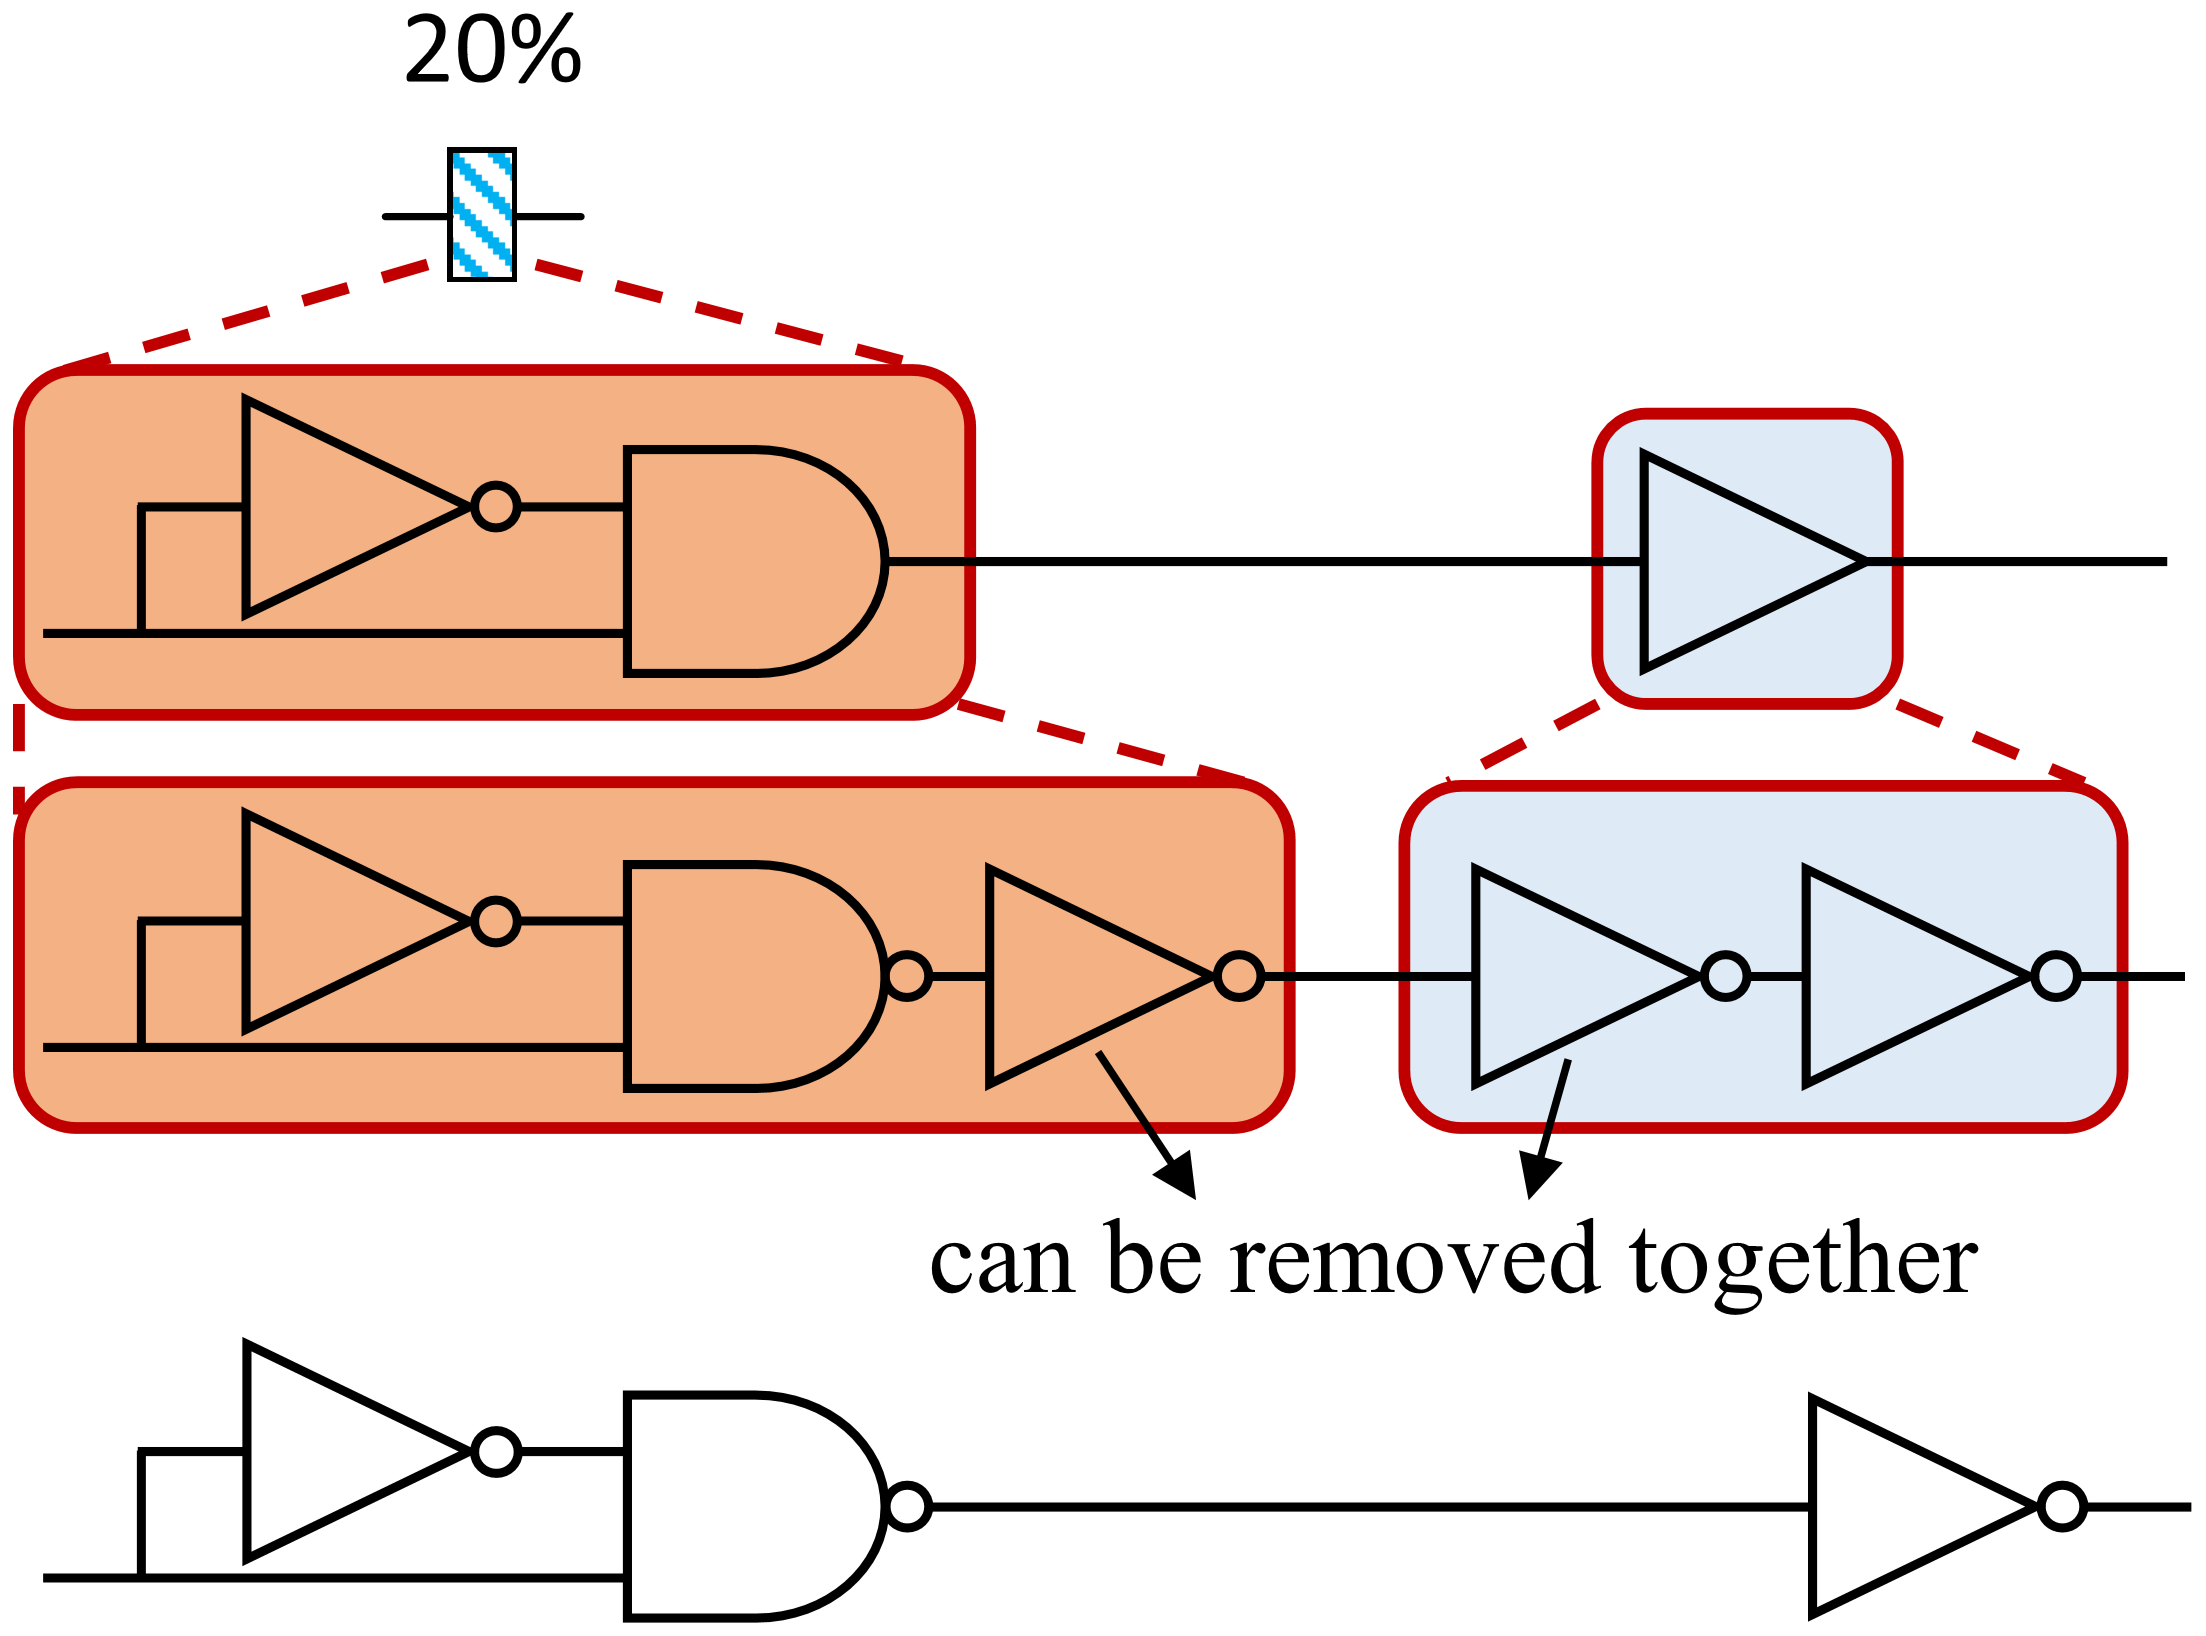
\includegraphics[width=0.5\columnwidth]{DCC_reduction.png}
    \caption{Practical considerations for DCC insertion}
    \label{fig:dccreduc}
\end{figure}

\subsection{Practical Considerations}
\label{subsec:tpc}
The diagram on the top of Figure~\ref{fig:dccreduc} shows the primitive design of a DCC, consisting of an inverter and an AND gate. In practice, the AND gate is implemented by a NAND gate feeding an inverter. As mentioned earlier, when inserting a DCC, it is inserted at the input of a buffer, which is a pair of inverters in practice. Therefore, we can actually use the diagram on the bottom of Figure~\ref{fig:dccreduc} to realize the insertion of a DCC. More specifically, we use it as a new cell to \enquote{replace} a buffer when a DCC is needed. By doing so, the cost of a single DCC can be significantly reduced and not much more expensive than the cost of inserting a buffer for clock skew scheduling. 